% vim:textwidth=70:lines=42
\chapter{引言}
\label{chap:intro}


%分布式管理系统的自管理方法研究
%分布式数据分发系统的优化方法研究
%系统层次结构任务模型的自动推断方法
%一种基于日志的任务层次结构推断方法


\section{选题背景}
% 管理和任务模型怎么捏到一起

% 分布式系统需要管理->管理=部署+维护(=监测+恢复)

% SMON维护应用的方法(online、offline、ignore)只是一种维护机制,可以
% 用于跑实验或长期服务的维护。维护机制可以有其他选择,例如可以没有(就
% 是ignore),可以用scalpel动态抓任务模型,看有没有正确性或者性能问题。

% 维护=监测+动作
% 监测:进程死活,应用内部状态等待
% 动作:重启?获取任务模型等等。

Internet服务正在改变着人们的生活方式。搜索引擎~\cite{google, yahoo,
baidu}改变了已有知识的组织与访问方式,它使得全世界的人们,可以通过互联
网方便地获取感兴趣的内容,这包括在线文档、图片、视频等内容,也包括更专
业的文献、新闻、金融信息、博客等搜索服务。除了搜索引擎,在线邮件~
\cite{gmail}服务让人们通过PC或者手机就可以随时随地处理自己的邮件。在线
文档~\cite{gdoc}服务使得人们不必安装专业软件,就可以创建、编辑与共享信
息。同时,多个个体可以协同编辑同一文档,而不必考虑底层的存储维护、一致
性保证等工作。在线交友~\cite{facebook}服务让人们有了新的互相认识与交流
的方式,它扩大了人们相互认识的途径,也改变了老朋友们维持友情的方式。

%其它Internet服务还有在线视频、照片。在线视频,交友,照片,博客。影响了
%其它产业,例如手机

支撑这些Internet服务的是一些大规模的分布式系统。分布式存储系统~
\cite{gfs, bigtable, dynamo}可靠的保存着回答搜索请求所需要的巨大容量的
信息,例如网页、图片、视频、地理信息、金融数据等。从而保证了在任何时间
、任何地点的人们,都可以有效地查询信息。内容分发网络~\cite{akamai,
coral}(CDN,Content Distribution Network)将网络服务“推送”到离用户
最近的网络边缘,这样,用户就能够就近快速访问服务,同时减轻了服务提供者
的负载。基于P2P覆盖网络的系统被广泛的应用在文件分发、共享~
\cite{bittorrent, sharkfs},视频组播~ \cite{chainsaw, coolstreaming,
bullet, splitstream}等服务。P2P覆盖网络让用户能够相互共享与分发数据,
从而有效提高了网络资源的利用率,同时减轻了服务器的压力。在学术界与工业
界,人们也在尝试使用P2P技术,搭建具有高度可扩展性和稳定性的存储系统,
提供“云存储”~\cite{s3, idisk}(Cloud Storage)服务。

早期的Internet服务基于单机系统。世界上最早的搜索引擎
Archie~\cite{archie}起初只使用了一台机器,它定期从一组FTP服务器获取文
件列表,为用户提供文件查询服务。随着用户越来越多,Archie逐渐从单机系统,
演变成由前端和后端组成,在Internet上有多处服务器的分布式系统。

随着Internet服务的普及与流行,支撑它们的分布式系统规模变的越来越大。以
Google为例,2006年\footnote{Google有意保密其系统规模等参数,因此难以获
得最新数据}的数据~\cite{how_google_works}表明,支撑Google服务的集
群规模已经达到了450000台机器,其耗电量达到了20兆瓦特,平均每月电费在
200万美元的规模。在2008年召开的Google I/O会议上,Google Fellow Jeffrey
Dean披露说,最大的BigTable运行实例运行在数千台机器上,存储了超过6
petabytes的数据~\cite{cnbeta_bigtable}。

% 现在,cluster规模: 450,000, 2006,how google works, wiki:google
% platform

有若干因素使得Internet服务必然选择分布式系统作为关键组成部分。首先,
Internet服务的成功,吸引了众多使用者。服务不再可能使用单机或者小规模集
群就能够胜任。随着普通计算机元件造价越来越低,人们可以很容易的搭建出规
模上千的分布式系统。用户请求被分散到不同的机器并行处理,提高了服务的吞
吐率与处理延迟。服务还会被分布到不同地区,使用户能够就近访问,减小了服
务的处理延迟。

其次,是为了保证服务的可靠性与可用性。用户希望服务总是可用的,也就是服
务总是可以访问的。同时,服务也应该是可靠的,用户的数据不应该丢失。因此,
系统使用冗余机制,将数据与服务复制多份。即便遇到故障,仍然能够处理用户
请求。

最后,有些Internet应用,其本身就必须是分布式系统。例如,基于P2P的文件
共享,视频组播等。只有分布式系统,能够将世界各地的用户连接到一起。CDN
服务也需要在全球部署服务器,将内容推送到网络的边缘。这些应用的本质决定
了使用分布式系统的必要性。

%\note{上面的内容还可以再扯一扯}

随着分布式系统被广泛应用,它也迅速成为了工业界与学术界的关注热点,对分
布式系统的研究热潮也一直持续着。一些重要的研究内容包括:分布式存储系统~
\cite{gfs, bigtable, dynamo, pacifica},并行编程模型~\cite{mapreduce,
sawzall, dryad, dryadlinq},分布式锁服务~\cite{chubby},分布式系统设计
方法与设计模式~\cite{sinfonia, boxwood, seda, mace, macedon, p2}等等。

\section{分布式系统运营准备}
% 存储gfs,big, dynamo,pacifica, exe engine mapreduce sawzal dryad
% dryadlinq,lock service(chubby)
% building block?sinfonia,boxwood,seda,paxos
% language approach: mace, p2

% 后面应该再想想,怎么引出问题。

时至今日,设计一个支持Internet服务的分布式系统仍然是困难的。分布式系统
设计日趋复杂的主要原因是为了高效处理流量巨大的用户请求,导致其规模越来
越大,并带来了一系列问题。为了处理日趋增加的用户请求,系统将请求分布在
不同机器、进程和线程间并发处理,使用异步消息机制协调任务的处理过程。用
来满足用户请求的数据其容量是巨大的,分布存储在不同的机器,需要使用冗余
机制提高分布式存储性能与可用性。由于使用了冗余机制,同时需要考虑一致性
问题。分布式系统还需要应对频繁发生的机器故障和网络故障。同时解决上面这
些挑战,设计出一个稳定正确运行、可扩展性好、性能优良的分布式系统是相当
不容易的。

\begin{figure}[htbp]
\centering
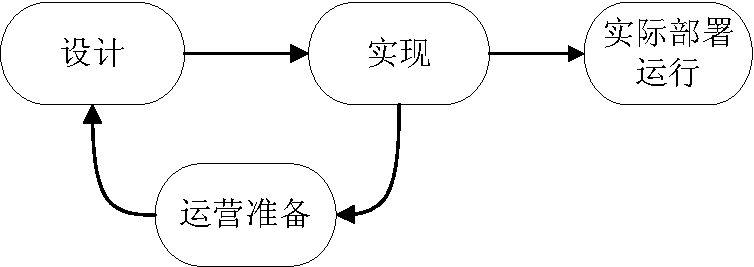
\includegraphics[width=0.6\linewidth]{op}
\caption{分布式系统设计实现与运营准备的迭代过程}
\label{fig:op}
\end{figure}

分布式系统的规模和复杂性导致了在正式上线之前,需要经过运营准备阶段,试
验性的运行系统并调试解决可能的问题,虽然很难设计出完全正确与性能优异的
系统,但是人们总是希望将出错的可能性降到最底,并尽量使系统性能最优。如
图~\ref{fig:op}所示,通常一个分布式系统要经过多次“设计$\to$实现$\to$
运营准备$\to$重新设计”的循环,逐步改进系统设计与性能,才能最终在生产
环境部署运行。

运营准备是一个传统的概念。通常,为保证一项工程或产品在设计生产后能够正
确而稳定的执行预期的功能或任务,需要执行一定的准备工作,这些工作称为运
营准备工作。不同的系统其运营准备各不相同,需要结合系统自身的特点与用途
确定运营准备工作的内容。例如,Microsoft BizTalk的运营准备过程包括如下
内容:配置Windows操作系统、IIS服务器、SQL Server服务和BizTalk服务器,
高可靠性与容错配置、备份与灾难预防、监控、系统测试等诸多任务。

分布式系统运营准备从狭义来说是确保系统本身能够正确且高效的工作,从广义
角度来说,甚至包括机房建设与布局、机房环境控制、开发维护人员的培训、电
力保障等很多内容。即使是从狭义的角度,分布式系统运营准备也包含如下一些
工作:

% 最好有个复杂的图

\textbf{管理分布式系统运行}:分布式系统的规模决定了管理工作的难度,由
于支撑Internet服务的分布式系统规模通常很大,其管理工作也面临诸多挑战。
分布式系统管理分几个方面,首先需要将系统部署在一组机器上。分布式系统需
要被部署到每个机器上,正确配置运行环境,并被安装启动。其次,需要监测系
统的运行状态,最基本的要求是监测应用的节点是否在运行,如果由于各种原因
应用的某些节点运行失败,管理系统应当尝试自动恢复运行失败的部分,并依据
一定配置报告失败事件。目前,管理系统需要面对相比以前规模更加巨大的分布
式系统,以往的设计在这样的规模下存在可扩展性和容错等新的问题。由于管理
系统规模也在增大,因而本身的自管理、扩展性、容错等问题也凸显出来。

\textbf{检测系统设计}:分布式系统运行在异步网络环境中,需要正确的处理
所有可能的异步消息顺序,也要考虑频繁发生的来自网络、节点、应用层次的所
有可能错误。在测试阶段,需要在不同的层次,测试系统在所有可能的消息内容
、消息顺序、错误类别组合下,仍然能够正确运行。除了测试系统执行逻辑的正
确性,还要测试系统的性能,以保证系统能够负担大规模的用户访问。

\textbf{调试系统缺陷} :通常在运营准备阶段,会发现系统的逻辑性错误和性
能问题,统称为系统缺陷。在发现问题后,需要追踪产生问题的原因,并重新实
现或设计系统。分布式系统的规模和复杂性让调试分布式系统的正确性与性能缺
陷面临很多困难与挑战。分布式系统将任务,例如用户请求,分为不同的阶段执
行,这些阶段可能被分散到系统的不同节点、进程和线程中处理,其执行顺序可
能是并行也可能是串行的。不同阶段之间,使用信号、异步消息作为通知机制。
传统的调试方法很难跟踪与分析分布式系统的运行时行为。

%其中的难题是xxx,我们研究的内容主要是xxx,意义与困难?

本文分别研究了分布式系统运营准备中的若干关键问题,集中在分布式系统管理
与调试两方面。下面分别叙述这两方面研究的重要问题,并在~
\ref{sec:intro_contrib}节引出本文的研究内容与贡献。

% (重写,管理概述)与传统单机软件不同,分布式系统需要被有效地管理。分布
% 式系统由运行在不同机器上的应用节点组成,应用节点通过网络相互连接,共同
% 完成设计的功能。因此,需要首先将系统部署到一组机器上才能运行。这其中的
% 核心问题是如何将应用分发到规模成百上千台机器上去,考虑到系统规模巨大,
% 同时各种故障随着规模增大而频繁发生(例如机器故障、网络连接断开),因此
% 部署一个分布式应用并不容易。在应用部署并启动之后,它的运行状态需要被紧
% 密监测,以保证系统运行正确、稳定,性能达标。
% 
% (类似管理概述,调试概述)分布式系统的调试也是个挑战。规模大,并行处理,
% 请求经过不同节点,异步处理,更复杂的逻辑,错误处理。(或者应该说调试研
% 究什么,而不是研究的难点。)
% 
% 
% 本文分别研究了分布式系统管理与调试中的关键问题。具体的,针对xxx我们研
% 究了xxx。
% 
% 接下来,我们首先对xxx研究的基本内容做概要叙述,并在xxx节叙述本文的主要
% 研究内容,包括研究的问题、挑战与基本解决方法,以及本文研究成果的
% 目标使用者,以及本文的主要贡献。

% 从历史看分布式系统发展的脉络,从应用看分布式系统使用的必然性

% 随着系统规模越来越大,设计一个分布式系统遇到了新的问题与挑战。


% 与单机运行软件不同,一个分布式系统在设计与实现之后,如何管理与调试也面
% 临着诸多挑战。

% 1. motivate 管理和调试
% 2. 管理和调试捏到一起
% 3. current limitation

% \subsection{Internet服务与分布式系统}
% 
% 这章或许可以不要,等写完了下面章节的内容再回来看看。
% 
% 这章其实就是扯淡,主要述说了Internet服务中的分布式系统都有什么,各有什
% 么特点。
% 
% \subsection{分布式系统设计}
% 
% 设计一个分布式系统需要解决许多困难问题,通常下面这问题是必须考虑的:
% 
% 可扩展性;可靠性;容错;一致性;可扩展性

\subsection{分布式系统管理}
\label{sec:intro_mgmt}

分布式系统或分布式应用\footnote{在后面的叙述中,我们交叉使用“分布式系
统”或“分布式应用”来表达相同的意思。}管理包括若干问题。分布式系统需
要运行在由网络连接的一组机器上,不同的系统对机器、网络资源配置的要求也
不同。我们需要在分布式计算平台提供的资源基础上,选择出一个符合要求的子
集,这就是\emph{资源发现}。其次,需要将分布式系统\emph{部署}到这组机器
上,包括分发系统的安装程序,在每个机器上配置运行参数,并在各个机器启动
系统运行。在系统运行期间,需要\emph{监测}系统运行状态。这包括对系统所
在计算平台的监测,也包括对系统本身状态的监测。最后,管理者希望能够自动
将系统从运行失败中恢复,并动态的控制系统的运行等。

本质上,分布式应用管理系统也是一个分布式应用。由分布在许多机器上的管理
节点构成。节点通过相互合作,共同完成管理任务涉及的信息收集(资源发现)
、数据分发(部署)与数据聚集(监测)等工作。随着被管理分布式系统规模越
来越大,管理系统在完成管理任务的同时,自身也需要考虑自管理、可扩展、容
错等问题。

\subsubsection*{资源发现}

支撑分布式系统运行的分布式计算平台规模可能非常大,
Planet-Lab~\cite{Bavier2004}包括了超过1000个分布在Internet上的节点,而
Google使用的集群规模达到了数万台机器。通常一个分布式系统并不需要使用计
算平台上的所有机器。开发者或者管理者需要找到满足系统运行的一组资源,包
括一组机器以及连接这些机器的网络。

不同的分布式系统对资源的要求不同。科学计算程序希望能够找到空闲CPU与内
存都很大的机器,如果计算过程中有频繁的数据交换,那么这些机器之间的网络
连接状况也应该很好。一些科学计算程序运行时间较短,从几小时到几天。因此
它们更关心资源的当前使用情况。还有一些分布式系统提供长期的服务,例如资
源发现服务本身。它们定期收集计算平台的资源使用情况,并执行来自用户的查
询。这些服务并不需要使用很多CPU与内存资源,但是它们希望运行在长期稳定
的一组机器上,频繁的机器或网络故障会影响服务的质量。

资源发现服务~\cite{sword_toit, xenosearch}接受用户对所期望资源的描述,
并返回满足要求的一组资源,如果没有资源能够满足用户的期望,则返回空。抽
象来说,这是一个图的匹配问题。资源发现服务定期收集整个分布式计算平台的
资源使用数据,包括每个机器的计算资源和存储资源等,以及机器之间网络连接
情况,将其以适合的方式保存。用户将对期望资源的描述用图的形式表达。图的
节点描述了机器应当满足的条件,图的边描述了机器之间的网络连接应当满足的
条件。资源发现服务要在整个计算平台这个大图上,寻找满足用户条件子图,这
等价于k-clique问题,是一个NP-hard问题。

\subsubsection*{部署}

部署是将分布式系统分发、安装到选定的一组机器上,并配置、启动系统运行的
过程。其核心是如何将系统分发复制到一组机器上。可以使用集中式的方法部署
分布式应用~\cite{vxargs, pssh}。管理者从一个集中控制机器,将系统的安装
程序远程复制到各个机器上,并逐个配置、启动应用的进程。这种方法最大的优
点是设计实现简单,许多情况下,只需要编写几个脚本就可以完成绝大多数工作。
集中式的方法对小规模应用很有效,但是却不能很好的胜任大规模时的情况。首
先它的可扩展性很差,在部署多台机器时,所有的数据都通过本地网络分发,效
率低下。其次,在大规模情况下,网络与机器故障成为频繁发生的事情。集中式
方法使用的静态星型拓扑结构不能很好的处理这些故障。

因此,各种基于P2P算法的部署工具~\cite{bittorrent, codeploy, sharkfs}被
研究并开发。这些工具本身也是一个分布式系统,由运行在不同机器上的节点构
成。节点通过相互合作,从对方获取自己没有的数据块,从而有效地节省了数据
源所在节点的网络资源。同时,这些工具能够动态的适应网络环境的变化,选择
最佳的数据传输路径,从而提高了部署的效率,同时也能有效地应对一些网络故
障。依据节点间形成的网络拓扑结构,可以将工具分为基于随机结构网络拓扑的,
或者基于结构化网络拓扑的。

一些复杂的分布式应用通常由多种类型的节点构成。例如一个典型的三层结构的
Web应用,由前端的Web服务器,中间的应用处理和后端的数据存储构成。每一层
都可能是一个分布式系统。为了有效地支持这种复杂的部署需求,一些功能上更
先进的部署工具被研究并开发出来~\cite{plush, smartfrog}。这些工具提供了
与自身绑定的描述语言,使用者使用描述语言给出部署说明,工具能够自动完成
指定的部署任务。

\subsubsection*{监测}

分布式系统的运行状态散布在各个机器,人们需要监测系统的运行状态。这包括
底层计算平台的状态~\cite{comon},与应用本身的状态。所监测的状态指标有
表示系统是否正确运行的,也有表示系统运行性能的。

在许多情况下,监测的目标并不是针对每个机器或者每个应用进程,而是针对所
有状态的一个聚集运算。例如,返回所有CPU使用率超过95\%的前十个机器列表。
最直接的办法是将所有状态集中收集到一起,然后进行计算。然而这样的方式扩
展性太差,在实际中没有可操作性。一些算法~\cite{sdims, somo, sanfermin}
使用树的结构,将需要聚集的属性从树叶向上传递,树中的节点将子节点的结果
聚集后再向上传递,因此减少了数据的传输。还有一些系统~\cite{astrolabe}
使用基于epidemic和gossip的算法,通过节点之间随机的交换数据,达到统计意
义上保证一定准确率的聚集结果。

使用聚集的方式可以持续监测某个全局状态的值,但是在一些情况下,人们只想
在知道全局状态是否满足一些约束谓词。例如,从每个机器访问任意站点的流量
总和不能超过100M/s,这是监测DDoS攻击的一个全局约束。在这种情况下,我们
不需要持续的聚集每台机器的流量状况。针对这种需求,可以使用分布式触发器
(distributed trigger)~\cite{Jain2004, Huang2006, Keralapura2006,
Sharfman2007, Cormode2005, Das2004}技术。这种技术在约束没有被违反的情
况下并不传输任何数据,因此进一步降低了监测所带来的流量负载。

\subsection{分布式系统调试}
\label{sec:intro_debugging}

分布式系统是Internet应用的关键组成部分。然而分布式系统很难设计与实现,
并且很容易包含错误(bug)。分布式系统将用户请求在很多机器上并发处理,
其目的是为了提高处理效率。然而并行程序不容易编写,需要考虑更多的运行状
态与处理逻辑。并行程序通常使用异步通信,以提高性能。因此消息可能是乱序
的,或者被丢弃。这使得处理逻辑更复杂。另外,在大规模系统中,机器与网络
故障是频繁发生的事件,分布式系统需要考虑到各种可能的情况并很好的处理。
考虑到以上这些困难,设计一个运行正确,并且可扩展性好、稳定、性能良好的
分布式系统是有相当挑战性的。

分布式系统的错误大致可以分为两类,正确性错误与性能问题。一个正确性错误
的例子是,在一个采用主从结构设计的分布式存储系统中,任何时刻只能有一个
主要节点。如果一些未考虑的事件序列,导致系统产生了两个主要节点,那么系
统就产生了正确性错误。性能问题的例子是,在一个搜索引擎服务中,前端服务
器接到用户搜索请求,将请求分发给后端的多个索引服务器,等所有的索引服务
器都返回后,将搜索结果返回给用户。然而,索引服务器的工作进度有快有慢,
因此整体的搜索性能受到最慢的索引服务器限制。在某些情况下,有的索引服务
器返回结果的时间很长,造成了性能问题。

分布式系统的错误难于调试,产生错误的原因深藏在系统复杂甚至是混乱的逻辑
与实现中。目前,设计分布式系统尚缺乏形式化方法支持,因此搭建分布式系统
更像是艺术,设计者凭借自己的经验进行设计,然而总会有超出经验的错误发生。
目前,有以下一些分布式系统调试的方法。
% 然而异步发生的消息传输与错误事件,使得可能的系统状态爆炸性增长。

\subsubsection*{基于因果路径(causal path)的方法}

% 基于因果路径?任务模型是一个扩展

% 这种方法的基本思想是使用任务模型描述分布式系统的运行时行为,从而人们可
% 以使用任务模型理解、验证和分析分布式系统的设计与实现。

分布式系统将任务,例如一个用户请求,分为不同
的阶段执行,这些阶段可能被分散到系统的不同节点、进程和线程中处理,其执
行顺序可能是并行也可能是串行的。不同阶段之间,使用信号、异步消息作为通
知机制。传统的调试方法很难跟踪与分析分布式系统的运行时行为。

\begin{figure}[htb]
\centering
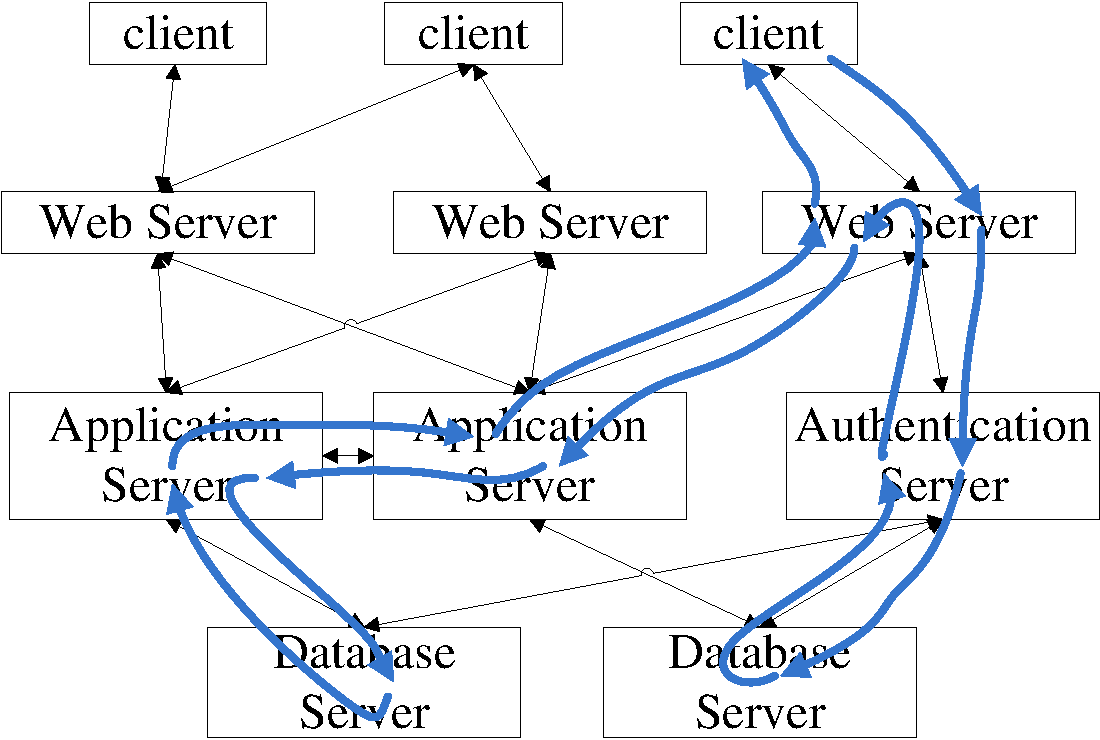
\includegraphics[width=0.6\linewidth]{3tier_causalpath}
\caption{三层结构Web服务处理用户请求的因果路径示例}
\label{fig:3tier}
\end{figure}

可以使用因果路径描述与分析分布式系统运行时行为~\cite{pinpoint, magpie,
pip, x-trace, project5}。一个任务的执行过程,可以抽象为一个因果路径。
因果路径包含了一组有偏序关系的事件集合。事件对应任务执行过程的某个阶段,
事件的偏序关系对应阶段之间的因果依赖关系。因果关系可以分为两种,两个阶
段被顺序执行而产生的因果关系,以及两个线程使用信号、异步消息等通知机制
而产生的依赖关系。图~\ref{fig:3tier}显示了一个典型的三层结构Web服务在
处理一个用户请求时产生的一条因果路径。用户请求到达Web服务器,Web服务器
首先向认证服务器发消息,认证服务器在读取数据库后返回认证结果。接着,
Web服务器向应用服务器发送消息,应用服务器将消息发送给另外一个应用服务
器,后者在读取数据库后返回消息处理的响应。第一个应用服务器将响应返回给
Web服务器,响应最终到达用户。

每个因果路径都由某个外来的“刺激”触发,用户请求是常见的一种。其它情况
还包括由定时器(timer)触发的系统内部维护任务,以及由错误事件触发的错
误处理任务。

使用因果路径描述系统运行时行为需要解决两个主要困难。首先,需要将每个事
件与所属的任务关联。分布式系统通常使用了线程复用机制(线程池)处理任务。
这导致同一个线程在不同的时间段会执行不同的任务,线程与任务之间有多对多
的关系。其次,需要得到联系事件之间的因果依赖关系。分布式系统运行时并发
产生许多的异步消息、信号等通信,将它们记录下来,并正确的将事件相匹配并
不容易。

在得到系统运行时的一组因果路径后,我们可以对系统行为进行分析。包括验证
每个因果路径是否有正确的结构(例如执行顺序、依赖关系是否正确),是否有
正确的性能(例如执行时间、延迟是否达标)等等。

% 可以将分布式系统的运行时行为用任务模型来描述。任务模型描述了任务的执行
% 路径。任务模型可以用图来描述,包含两部分,组成任务执行过程的子任务,和
% 子任务之间的因果依赖关系。子任务是图上的节点。子任务之间边对应的它们之
% 间的依赖关系。子任务因为使用信号、异步消息等通信机制协调运行顺序,而产
% 生因果依赖关系。
% 
% 使用任务模型描述系统运行时行为需要解决两个主要困难。首先,需要标记合理
% 的任务边界。分布式系统通常使用了线程复用机制(线程池)处理消息与事件。
% 这导致同一个线程在不同的时间段会执行不同的任务,线程与任务之间不存在一
% 一对应关系。因此,需要将线程的执行过程分为不同的片段,每个片段属于一个
% 任务的执行过程。其次,需要正确的联系任务之间的因果依赖关系。分布式系统
% 运行时并发产生许多的异步消息、信号、事件等通信,将它们扑捉并正确的与相
% 关联的任务配对并不容易。


\subsubsection*{基于谓词检查的方法}

可以使用谓词来检查分布式系统的不变量~\cite{d3s}。虽然分布式系统非常复
杂,但是其主要性质可以用少数几个不变量来描述。例如,对一个主从结构的分
布式存储系统过来说,一些主要的不变量包括,数据副本一致性,任何时刻只能
有一个主要节点。只要这些不变量能够保持,系统就能够正确运行。

使用谓词检查分布式系统,首先需要动态提取计算谓词需要的系统状态,这些系
统状态分布在不同的节点和进程内。常见的技术是使用动态插装,将系统状态暴
露给外界。将状态汇总后,可以计算谓词是否满足。计算在系统状态的一组一致
快照(consistent snapshot)上进行检查。在谓词取值为假时,表示系统不变
量被打破,发生了错误。通过检查导致谓词从真到假这一过程的相关状态,可以
帮助找到问题产生的原因。在设计谓词检查一个大规模系统时,同时要考虑到自
身的可扩展性和容错。可以使用层次结构的方式将谓词的计算结果逐步汇聚。使
用错误检测器探测失败的谓词计算进程。

\subsubsection*{基于回放的方法}

分布式系统的错误通常依赖于一组特定的事件序列,错误不是确定性的。在错误
发生后,重新运行系统并不会产生相同的结果。基于回放的方法~\cite{liblog,
friday, r2, mpiwiz}把系统运行过程中的事件、消息与它们的顺序都记录下来,
在错误发生后,能够重新“播放”错误发生的过程,直到错误原因被找到为止。

有两种回放的方法。数据回放方法记录了每个进程运行时收到的消息,在回放时
原样提供这些数据。数据回放记录的数据量很大,因为需要记录每一条收到的消
息,但是可以在回放时分别调试每一个进程,不用回放整个系统。顺序回放的方
法不记录消息的内容,只记录消息发送的顺序,保证在回放时系统能够确定性的
重播错误发生的过程。顺序回放记录的数据小,但是回放时需要重新运行整个系
统,消息的内容在系统运行时动态产生。\onlinecite{mpiwiz}的工作将数据回
放和顺序回放结合起来,在将节点按照通信量分为不同的组,组内通信量大,采
用顺序回放,组间通信量小,采用数据回放。这种方法结合了两种回放的优点,
使得每个组可以单独回放,不用启动所有的进程,同时记录的数据量也较小。

% causality, execution path and task model
% 
% predicate
% 
% replay
% 
% model checker
% 
% 
% 分布式系统设计复杂,是为了满足可扩展性等要求。对调试有了新的困难。
% 
% 分析分布式系统的复杂点
% 
% 任务模型的作用
% 
% 因果关系图?
% 
% 日志(一般性研究的方法,结果)
% 
% 基于对分布式系统运行状态监测的分析?


\section{本文研究内容与贡献}
\label{sec:intro_contrib}

本文研究了分布式系统运营准备中的若干关键问题,包括分布式管理系统的可自
管理方法、分布式数据分发的优化策略选择、自动推断层次结构任务模型方法和
基于日志的任务层次结构推断方法。

\subsection{研究内容}

\subsubsection*{分布式管理系统的自管理方法研究}

为了有效地管理大规模分布式应用,分布式应用管理系统也成为了一个复杂的分
布式应用,由散布在许多机器上的管理节点构成,共同完成应用的部署、监测与
错误恢复等任务。这就带来一个问题,作为一个分布式应用,管理系统也需要被
管理。需要部署管理系统的节点,监测其是否正常运行,并将系统从错误中恢复。
使用现有的技术,有两种解决这个问题的方法。其一、使用集中式方法管理使用
的管理系统。集中式方法易于实现,但是集中式方法扩展性差,对网络资源的利
用效率低,同时不能够很好的应对分布式环境下经常发生的网络异常。其二、使
用一个采用了P2P算法的管理系统去管理我们需要使用的管理系统。这个方法虽
然表面看上去很有效,但是新采用的管理系统又递归的产生了需要被管理的问题,
所以这个方案并没有解决问题。

在本文中,我们通过给管理系统增加内建的自管理能力,从根本上解决了管理系
统本身也需要被管理的问题。我们将这一想法实现为一个具备自管理能力的分布
管理系统SMON(Self-Managed Overlay Network)。构成这个系统的节点相互监
测运行状态,并相互管理维护。SMON能自动将自己部署到一组指定的节点上去,
也能够自动恢复运行失败的节点,同时能够在线将整个系统更新至新的版本。

设计SMON有如下的几个难题。首先是保证其自管理具有良好的可扩展性,其次,
为了支持自动部署,需要一定的安全机制保证系统节点能够自动与计算平台的机
器认证并登陆,完成远程部署与错误恢复的任务。最后,需要设计合理的应用管
理语意。

我们分别解决了这几个难题。首先,我们使用epidemic算法实现自管理机制。
SMON节点相互随机探测,并依据探测的结果,自动执行相互管理与维护任务,包
括在远程机器上部署新的SMON节点,恢复失败的SMON节点,更新自身至新的版本。
其次,我们使用了认证代理机制使SMON节点能够自动与计算平台的机器认证并登
陆。SMON节点将登陆认证过程中的挑战密文转发给认证代理,并返回认证代理求
解的应答密文给远程机器,从而完成自动认证的过程。同时,这一机制保证了用
户提供的认证信息不会泄露到认证代理外部。最后,SMON支持长期运行的
Internet服务管理语意,用户可以在SMON之上部署其它管理系统来扩展管理语意。

我们对SMON的设计进行的理论分析表明,SMON的设计具有良好的可扩展性和性能。
SMON的自管理操作时间随系统规模呈$O(\log N)$增长,自我部署中的额外负载
和节点收到维护消息的频率都是常数级别($O(1)$),并不随系统规模变化。在
Planet-Lab平台上的实际评测证实了理论分析的正确性。

\subsubsection*{分布式数据分发系统的优化策略选择}

数据分发技术是很多分布式应用的基础,包括部署分布式应用、文件共享和内容
分发网络等。解决数据分发的基本技术是将文件分为逻辑上连续的若干块,系统
用户或者节点交换相互拥有的文件块,而不是直接向数据源服务器请求数据。这
样做的好处有几点,首先降低了服务的压力,其次,这样的设计具有很好的可
扩展性,随着系统规模增大,总体的传输带宽也会增大。再次,文件块级别的操
作提供了更细粒度的负载均衡,从而系统节点能够动态的调整下载策略,绕开可
能的网络错误,以及获取更高下载性能。

现有工作表明,存在两种优化分发性能的途径。临近邻居选择方法让节点从网络
距离上近的节点那里下载数据块。节点从近处的邻居下载文件块的速度更快,从
而得到整个文件的时间更短,分发系统的整体性能也得到优化。动态上传带宽分
配使用了贪心策略,这种方法通过动态选择上传目标节点,并分配上传带宽,让
数据块更快的从一个节点分发出去,优化了局部传输性能,使得整体分发性能也得
到优化。

虽然已有工作已经指出这两种方法可以优化分发性能,但是尚未对它们在真实
Internet测量数据上的表现进行深入研究与验证,包括优化方法本身的效果、优
化参数选择、优化方法受数据块选择方法的影响和叠加不同优化方法的效果等。

%临近邻居参数选择(临近比率)没有真实Internet数据验证
%上传带宽:k的选择何时更接近最优
%数据块选择的影响
%合并两种优化的效果

本文通过在真实Internet测量数据上的广泛模拟测试,得到了如下结论:

\begin{itemize}

  \item 临近邻居优化方法可以提高分发性能。随着临近节点占节点邻居列表的
  比例越来越高,系统的分发性能也单调提高,在邻居列表完全使用临近节点时
  达到最优。

  \item 动态上传带宽分配策略使用贪心算法确定上传节点的数目,提高了分发
  的聚集吞吐量,其优化效果达到了局部最优。
  
  \item 两种优化方法对数据块选择策略敏感程度不同。邻近邻居选择优化依赖
  于LRF数据块选择算法,而上传带宽分配方法对数据块选择策略不敏感。

  \item 合并两种优化方法并不具有明显的叠加效果。实际应用中只需要选择一
  种优化方法应用。

\end{itemize}


\subsubsection*{系统层次结构任务模型的自动推断方法}

分布式系统难于调试。支撑Internet服务的分布式系统本质上非常复杂,这增加
了理解系统异常行为的难度。这些系统通常使用了分层的体系结构,将其功能抽
象表达为不同的层次结构。其运行时具有高度的并发性。系统在运行时,处理着
许多用户层次的\emph{任务},例如用户请求。任务被分成许多阶段,不同的阶
段被分布在多个机器、进程和线程上执行,使用事件或者异步消息作为通知机制。
验证单独每个任务的行为,是一件具有挑战性的问题,因为开发人员需要重构出
任务的执行流,将任务执行过程中的各个阶段重新连接起来。

从概念上说,开发人员可以把任务执行表示为\emph{层次结构的任务模型},这
与系统的分层体系结构设计一致。不同层次的任务表示在不同阶段不同模块执行
的一段执行过程。高层任务的执行被分为若干低层子任务。基于任务模型,开发
人员可以更好的理解系统模块间的结构,以及不同模块间的依赖关系,并验证处
于不同层次任务的行为。

已有工作需要开发人员手动标注任务模型。只有对系统的设计与实现非常熟悉的
专业人员才能正确的标注任务模型。针对这个问题,本文研究了一种自动推断系
统层次结构任务模型的方法。

推断方法应用在系统运行时trace上,我们使用同步点作为启发自动推断出叶子
任务的边界,叶子任务是任务模型中最基本的任务单位。然后,我们依据
happen-before关系推断出叶子任务之间的因果依赖关系,得到系统任务的因果
关系图。在这个因果关系图的上,我们使用图的聚类算法自动寻找频繁子图,将
叶子任务归纳为高层任务。通过递归使用聚类算法,我们得到了系统的层次结构
任务模型。

在一些复杂系统(Apache、PacificA)上的应用实例表明,推断方法能够自动推
断出具有合理含义的任务模型来,使用得到的任务模型,能够帮助理解与验证系
统设计,解决系统已有的性能问题。使用推断得到的任务模型帮助调试了
PacificA 分布式存储系统(类似BigTable)的性能问题,该问题使压力测试中
网络带宽利用率远低于100\%。


\subsubsection*{基于日志的任务层次结构推断方法}

% 任务层次结构?任务模型?

我们进一步研究了如何利用系统日志,推断系统任务层次结构的方法。与自动推
断系统层次结构任务模型的方法不同,这个工作基于系统运行过程中生成的日志。
其理念是,系统日志包含了更多的应用层任务流的语意。日志是由系统开发人员
创建的,因此它们包含了关键的系统状态和事件信息,例如,用户层任务的开始
和结束,处理用户请求的关键步骤等等。利用这些信息,可以帮助我们推断应用
层任务语意,而这些很难从系统运行trace中得到。

使用日志推断分层任务模型需要解决两个问题。第一、日志通常是非结构化的,
我们需要从中提取出和任务相关的信息。第二、推断任务之间的层次关系,构建
层次结构的任务模型。我们通过观察系统日志得到了一个提取任务信息的启发(
heuristic),使用这个启发,我们从日志中提取出了任务信息,包括任务的名
称与ID。接着,我们通过归纳任务之间的层次嵌套关系,推断出任务的层次结构
来。

我们实现了基于日志的任务模型推断工具,并使用它分析一个分布式存储系统
ChunkFS。ChunkFS是一个类似GFS~\cite{gfs}的分布式文件系统。我们的工具能
够推断出合乎逻辑的任务层次结构。应用推断的模型,帮助我们理解ChunkFS的
实际运行过程,并解决了ChunkFS中性能问题。经验表明,系统日志能够很好的
反映出上层语意,我们的推断方法可以有效的推断出系统任务模型,帮助理解系
统设计和运行时行为与调试系统性能问题。

\subsection{目标使用者}

本文针对分布式系统运营准备阶段的一些关键问题进行了一些研究,其研究结果
可以被以下三类使用者使用:

\begin{description}

  \item[系统开发者:] 系统开发者设计并实现系统,并负责调试与优化系统。他
  们对代码非常熟悉,知道系统运行时应该是什么行为。他们可以使用本文的工
  作验证系统设计是否正确,找到系统错误发生的根本原因。

  \item[系统代码维护者:] 系统代码维护者能够访问系统代码,但是对整个系
  统的设计并不熟悉。通常他们需要逐渐熟悉代码和系统设计。他们可以使用本
  文的工作理解系统的运行时行为,逐渐学习系统设计。

  \item[系统管理员:] 系统管理员通常不需要接触系统代码。他们可以使用本
  文的工作有效地管理分布式系统。通常,系统管理员需要监测系统是否运行正
  确,他们也可以使用本文工作监测系统运行时行为是否和预期一致。系统的正
  确运行时行为由系统设计和开发者提供。

\end{description}

\subsection{研究贡献}

本文研究的主要贡献和创新点是:

\begin{enumerate}

    \item 提出了使管理系统具备自管理机制的方法,设计实现了一个自管理的
    分布式应用管理系统SMON。SMON的自管理方法基于epidemic算法和认证代理
    技术,保证了自管理的可扩展性和安全性。理论分析表明,SMON的自管理操
    作时间随系统规模呈$O(\log N)$增长,自我部署中的额外负载和节点收到
    维护消息的频率都是常数级别($O(1)$),并不随系统规模变化。在
    Planet-Lab平台上的实际评测证实了理论分析的正确性。SMON支持长期运行
    的Internet服务管理语意,用户可以很容易的扩展需要的应用管理语意。

    \item 研究了分布式分发系统的优化策略选择问题。通过在真实Internet测
    量数据上的广泛细致评测,研究了邻近邻居选择与动态上传带宽分配两种优
    化。得到了如下重要结论:临近邻居优化效果随邻近邻居比率增加而单调增
    加,其优化效果依赖于LRF块选择算法;使用贪心算法确定的上传节点个数
    使优化效果达到了局部最优,并且不依赖LRF块选择算法;合并使用两种优
    化方法并不具有叠加优化效果。这些结论对实际系统应用具有重要指导意义。

    \item 提出了一自动推断系统层次结构任务模型的方法。解决了已有工作需
    要需要手动标注任务边界与依赖关系的问题。本方法使用同步点作为启发自
    动推断任务边界,使用happened-before关系作为启发自动推断任务因果依
    赖关系,使用图上的聚类方法自动推断系统任务的层次结构。在实际系统上
    的应用表明,推断出的任务模型能够帮助理解与验证系统设计,调试系统性
    能问题。使用推断方法帮助调试了PacificA分布式存储系统(类似BigTable)
    的性能问题,该问题使压力测试中网络带宽利用率远低于100\%。

    \item 提出了从系统日志中推断任务层次结构的方法。系统日志代表了系统
    运行时的活动,本推断方法能够自动从无结构的系统日志文本中提取任务信
    息,并在一组任务上推断任务之间的层次结构关系。使用得到的任务层次关
    系,可以将系统活动分为层次结构任务实例,帮助理解与验证系统设计,解
    决系统性能问题。使用推断方法帮助解决了ChunkFS(类似GFS)的性能问题,
    该问题使压力测试中网络带宽利用率远低于100\%。

\end{enumerate}

\subsection{内容组织}

本文主要研究了分布式系统运营准备中的关键问题,内容安排如下:

  第1章(本章):叙述了本文工作的研究背景,阐述了研究分布式系统运营维
  护的的必要性,并叙述了本文工作的动机、研究内容和主要贡献。

  第2章:叙述了分布式系统运营维护领域与本文相关的一些研究内容,包括相
  关研究的基本问题、方法和结果。

  第3章:研究了分布式管理系统的自管理方法,并设计实现了基于epidemic算
  法和认证代理结束的可自管理的分布式应用管理系统SMON。SMON具有内建自管
  理能力,包括自我部署、自我更新和自我恢复能力。SMON使用认证代理技术使
  节点能够安全的部署与恢复失败的其它节点。SMON支持长期运行的Internet服
  务应用管理语意。SMON有效的解决了管理系统也需要被管理的问题。理论分析
  和在Planet-Lab上的评测表明,SMON具有良好的性能与可扩展性。

  第4章:研究了邻近邻居选择和动态上传带宽分配两种数据分发优化策略的选
  择。首先给出了数据分发系统的一般模型,叙述了如何使用邻近邻居选择和动
  态上传带宽分配优化分发性能。通过在真实Internet测量数据上的广泛模拟测
  试,研究了两种方法的优化效果与优化参数选择、优化方法受数据块选择机制
  的影响和叠加两种优化方法的效果,并给出了在实际系统中应用的指导性建议。

  第5章:研究了自动推断系统层次结构任务模型的方法。通过使用插装技术透
  明的观测系统运行,获取系统运行trace,我们能够在不需要人手工帮助的情
  况下,自动推断出合理的层次结构任务模型。推断方法使用同步点作为启发自
  动推断任务边界,使用happened-before 关系作为启发自动推断任务因果依赖
  关系,使用图上的聚类方法自动推断系统任务的层次结构。实际应用经验表明,
  使用推断出的任务模型能够帮助我们理解系统设计,并解决系统的性能问题。

  第6章:研究了从系统日志中推断任务层次结构的方法。系统日志包含了更多
  的应用层任务流的语意,我们的推断方法能够自动从无结构的日志文本中提出
  任务信息,并推断任务之间的层次关系。使用推断出的任务层次结构能够帮助
  我们理解系统设计,并解决系统的性能问题。

  第7章:为全文做总结,并提出了一些进一步研究的方向。
